\section{Model}
The experimental setup we hope to model is shown in Figure \ref{expsetup}. The bars of the pendulum have significant mass so it is modeled as a compound pendulum. We will also include damping in the model in order to study its effects on the choatic behaviour of the system.

A schematic representation of the system is shown in Figure \ref{model}. Each bar $i$ is defined by a set of four parameters: $I_i$, the moment of inertia of the bar, $m_i$, the mass of the bar, $l_i$, the length of the bar, and $k_i$, the damping coefficient of the bar rotating about it's upper joint. The position and velocity of the bars are defined by the six system state variables: $\theta _1, \theta _2, \theta _3, \dot{\theta _1}, \dot{\theta _2},\dot{\theta _3}$. 

\begin{figure}[H]
\centering
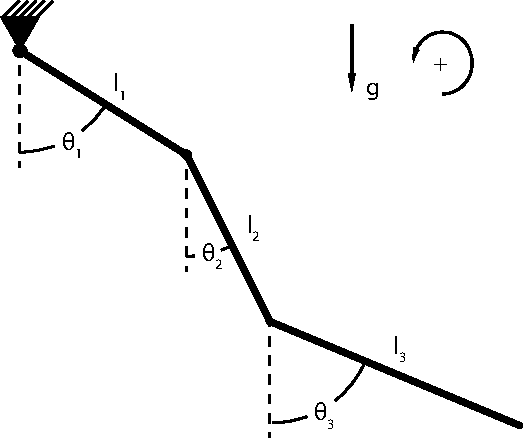
\includegraphics[scale=0.7]{Diagram.pdf}
\caption{Schematic representation of the model.}
\label{model}
\end{figure} 

We first derive the equations of motion of the frictionless ideal case. This allows for model validation by ensuring energy is conserved in the dynamics. Later we will add in frictional damping, and see how it changes the dynamics.

Taking down as +y and right as +x, we write the positions of the centers of mass of the bars as functions of $\theta _i$ and the geometric parameters of the system.

\begin{equation}
y_1 = \frac{l_1}{2}\cos \theta_1
\end{equation}
\begin{equation}
y_2 = l_1\cos \theta _1 + \frac{l_2}{2}\cos \theta_2
\end{equation}
\begin{equation}
y_3 = l_1\cos \theta _1 + l_2\cos \theta_2 + \frac{l_3}{2} \cos \theta _3
\end{equation}
\begin{equation}
x_1 = \frac{l_1}{2}\sin \theta_1
\end{equation}
\begin{equation}
x_2 = l_1\sin \theta _1 + \frac{l_2}{2}\sin \theta_2
\end{equation}
\begin{equation}
x_3 = l_1\sin \theta _1 + l_2\sin \theta_2 + \frac{l_3}{2} \sin \theta _3
\end{equation}

These positions are then differentiated with respect to time to find the x and y components of the velocities as functions of angles and angular velocities. They will not be shown here for brevity.

The magnitude of the velocity of each bar is
\begin{equation}
v_i = \sqrt{\dot{x_i}^2+\dot{y_i}^2}
\end{equation}
The translational and rotational kinetic energiy (TKE and RKE) of each bar is:
\begin{equation}
TKE_i = \frac{1}{2}m_iv_i^2
\end{equation}
\begin{equation}
RKE_i = \frac{1}{2}I_i\dot{\theta_i}
\end{equation}
The gravitational potential energy(GPE) of each bar is:
\begin{equation}
GPE_i = m_igy_i
\end{equation}

Using these, the Lagrangian of the system is:
\begin{equation}
\mathcal{L} = T-V = \displaystyle\sum_{i=1}^{3} TKE_i+RKE_i-GPE_i
\label{lagrangian}
\end{equation}

Equation \ref{lagrangian} can then be input to Lagrange's Equation:
\begin{equation}
\frac{d}{dt}(\frac{d\mathcal{L}}{\dot{q_i}})=\frac{d\mathcal{L}}{dq_i}
\end{equation}
where $\theta _i$ is used for the generalized coordinate $q_i$. This yields a system of three equations which contain the angular acceleration terms, omitted for brevity. The solution of this system of three equations and three unknowns yields the expressions for the angular velocities. We then numerically integrate these angular velocities to produce the path of the pendulum. A characteristic plot of the path is shown in Figure \ref{paths}. Energy is conserved in the undamped simulation, and the pendulum appears to behave as expected.  An animation of the system was also created and used to validate the results.  Videos of the animation are posted on YouTube for chaotic (\href{http://youtu.be/7lNIAdsInMg}{http://youtu.be/7lNIAdsInMg}) and periodic (\href{http://youtu.be/_THTgIZqDGQ}{http://youtu.be/_THTgIZqDGQ}) intial conditions.  With this validation of our basic methods, we add damping to the system. 

The bars of the experimental setup are thin, and the velocities are generally low, so we chose to model the system damping with a viscous drag caused by the angular velocity of the joints. This viscous form of drag can be modeled in Lagrangian mechanics with the Rayleigh Dissipation Function:
\begin{equation}
D = \frac{1}{2}(\displaystyle\sum_{i=1}^{3}k_i\dot{\theta _i}^2)
\end{equation}
Lagranges equation is the rewritten as
\begin{equation}
\frac{d}{dt}(\frac{d\mathcal{L}}{\dot{q_i}})=\frac{d\mathcal{L}}{dq_i}-\frac{dD}{d\dot{q_i}}
\end{equation}

This modified form of Lagrange's equation produces a system of three equations which contain the angular velocity terms, as above for the undamped case. Solving for the angular velocity terms produces the equations of motion shown in Appendix A.



